\chapter{Set Theory}
\label{chap:ch3}

In software engineering, we are constantly working with collections of things: users in a system, records in a database, or nodes in a network. Set theory provides the formal mathematical language to describe and manipulate these collections with precision and clarity. It is the bedrock upon which many core computer science concepts—from database query languages like SQL to data structures and algorithmic logic—are built.

This chapter introduces the fundamental principles of set theory. We will begin with the simple, intuitive idea of a set and explore the formal notation used to define them. We will then cover the essential relationships between sets, such as subsets, and the core operations used to combine them, including unions, intersections, and complements. These operations directly correspond to the logical operators (\texttt{OR}, \texttt{AND}, \texttt{NOT}) that govern the flow of your code. Finally, we will explore ordered collections called tuples and introduce a simple method for proving set equalities.

\section{What is a Set?}
A set is an unordered collection of distinct objects. The objects within a set are called its \textbf{elements} or \textbf{members}. We can think of a set as a simple container where items are grouped together, and the order in which we list them does not matter. For example, the set of primary colors can be written as $\{ \text{red}, \text{yellow}, \text{blue} \}$ or equally as $\{ \text{blue}, \text{red}, \text{yellow} \}$.

Sets are a cornerstone of modern mathematics and a fundamental concept in computer science. They form the logical basis for everything from database query languages and data structures to the specification of programming language types.

% --- Figure Placeholder ---
% This figure illustrates the basic concept of a set.
% It is inspired by Slide 3 of your PowerPoint presentation.
\begin{figure}[htbp]
    \centering
    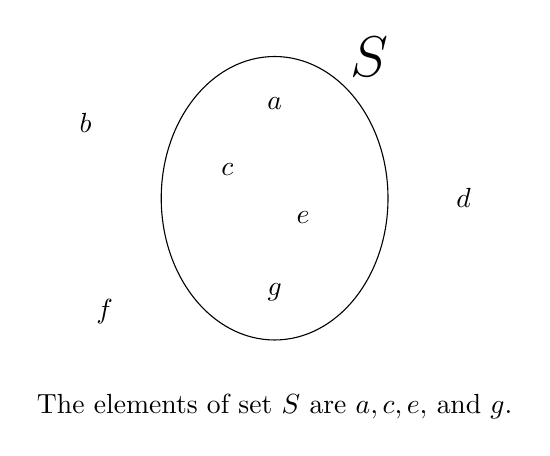
\begin{tikzpicture}[scale=1.2]
        % The set S as an ellipse
        \draw (0,0) ellipse (1.2cm and 1.5cm);
        \node at (1, 1.5) {\huge $S$};
        
        % Elements inside the set S
        \node at (0, 1) {$a$};
        \node at (-0.5, 0.3) {$c$};
        \node at (0.3, -0.2) {$e$};
        \node at (0, -1) {$g$};
        
        % Elements outside the set S
        \node at (-2, 0.8) {$b$};
        \node at (-1.8, -1.2) {$f$};
        \node at (2, 0) {$d$};

        % Annotation
        \node[align=center] at (0,-2.2) {The elements of set $S$ are $a, c, e,$ and $g$.};
    \end{tikzpicture}
    \caption{A set $S$ containing four elements. The objects $b, d,$ and $f$ are not elements of $S$.}
    \label{fig:set_concept}
\end{figure}

\subsection*{Specifying a Set}
There are two primary ways to describe a set: by explicitly listing its members or by defining a property that its members must satisfy.

\subsubsection*{Listing Notation (Roster Method)}
The most direct way to define a set is by listing all its elements between curly braces, $\{ \}$. This is known as the \textbf{roster method}.

For example:
\begin{itemize}
    \item The set of the first five letters of the alphabet is $A = \{a, b, c, d, e\}$.
    \item The set of the first three positive integers is $C = \{1, 2, 3\}$.
    \item A set can contain different types of elements: $D = \{ \text{Alice}, 42, \pi \}$.
\end{itemize}

When using the roster method, there are two fundamental rules:
\begin{enumerate}
    \item \textbf{Order does not matter.} A set is defined only by the elements it contains, not by the sequence in which they are listed. For example, $\{1, 2, 3\}$ is the exact same set as $\{3, 1, 2\}$.
    \item \textbf{Each element must be unique.} An element is either in a set or it is not. Listing an element more than once is redundant and does not change the set. For instance, the set $\{a, a, b, c, c\}$ is simply $\{a, b, c\}$.
\end{enumerate}


\subsubsection*{Set-Builder Notation}
When listing every element is impractical or impossible (for example, with infinite sets), we use \textbf{set-builder notation}. This method defines a set by stating a property or rule that its elements must satisfy. The notation uses a vertical bar `|` or a colon `:`, which is read as "such that."

The general structure is:
\[ \{ \text{variable} \mid \text{a property the variable must satisfy} \} \]

For example:
\begin{itemize}
    \item $A = \{ l \mid l \text{ is a vowel in the English alphabet} \}$ \\
    This is read as: "$A$ is the set of all elements $l$ such that $l$ is a vowel." This is another way of writing $A = \{a, e, i, o, u\}$.
    
    \item $C = \{ n \mid n \in \mathbb{Z} \text{ and } 0 < n < 4 \}$ \\
    This is read as: "$C$ is the set of all numbers $n$ such that $n$ is an integer and $n$ is greater than 0 and less than 4." This defines the set $\{1, 2, 3\}$.
    
    \item $E = \{ x \mid x \text{ is an even integer} \}$ \\
    This defines the infinite set of all even integers: $\{\dots, -4, -2, 0, 2, 4, \dots\}$.
\end{itemize}

Set-builder notation is extremely powerful because it allows us to define large, complex, or even infinite sets with a short and precise description.

\section{Important Sets: The Number Systems}
Numbers are the foundation of mathematics and computation. The different categories of numbers we use every day, from counting items to measuring continuous values, can be formally defined as sets. Understanding these fundamental sets is crucial for any software engineer, as they underpin data types, arithmetic logic, and numerical algorithms.

\subsection*{The Main Number Sets}
The following sets are some of the most important in mathematics and are used throughout science and engineering.

\begin{description}
    \item[Natural Numbers ($\mathbb{N}$)] The set of positive integers used for counting: $\{1, 2, 3, \dots\}$. Sometimes, this set is defined to include $0$. Due to this ambiguity, it is often clearer to specify \textit{positive integers} or \textit{non-negative integers}.

    \item[Integers ($\mathbb{Z}$)] The set of all positive and negative whole numbers, including zero: $\{\dots, -2, -1, 0, 1, 2, \dots\}$.

    \item[Rational Numbers ($\mathbb{Q}$)] The set of all numbers that can be expressed as a fraction $\frac{p}{q}$, where $p$ and $q$ are integers and $q \neq 0$. This includes all integers and terminating or repeating decimals. Examples: $\frac{1}{2}$, $-5$, $0.25$.

    \item[Real Numbers ($\mathbb{R}$)] The set of all numbers on the number line. It includes both rational numbers and irrational numbers (like $\pi$ or $\sqrt{2}$), which cannot be expressed as simple fractions.
    
    \item[Complex Numbers ($\mathbb{C}$)] The set of all numbers that can be expressed in the form $a + bi$, where $a$ and $b$ are real numbers and $i$ is the imaginary unit, satisfying $i^2 = -1$.
\end{description}

Visualizing the relationships between these sets is key to understanding them. A Venn diagram shows the hierarchy of how these sets are nested within one another, while a number line illustrates how they cover or populate the continuum of values.

% --- Venn Diagram of Number Systems ---
% This is the TikZ code you provided for the number system Venn diagram.
\begin{figure}[htbp]
    \centering
    \begin{tikzpicture}[scale=0.7]
        % Complex Numbers (outer square)
        \draw[thick, fill=lightgray!50] (-12, -6) rectangle (10, 5);
        \node at (8, 4) {\Huge $\mathbb{C}$};
        
        % Real Numbers (largest set)
        \draw[thick, fill=mseViaBlue] (-4,0) ellipse (7.8cm and 4.5cm);
        \node at (-3, 3) {\Large $\mathbb{R}$};
        
        % Rational Numbers
        \draw[thick, fill=mseOrange] (-7,0) ellipse (4.5cm and 3cm);
        \node at (-11, 0) {\Large$\mathbb{Q}$};
        
        % Integers
        \draw[thick, fill=mseDarkText] (-7,0) ellipse (3cm and 2cm);
        \node at (-9.5, 0) {\Large$\mathbb{Z}$};
        
        % Natural Numbers
        \draw[thick, fill=mseAnswerBg] (-7,0) ellipse (2cm and 1.2cm);
        \node at (-7, 0) {\Large$\mathbb{N}$};
        
        % Irrational Numbers
        \draw[thick, fill=mseQuestionBorder] (1,0) ellipse (2cm and 1.2cm);
        \node at (1, 0) {\Large$\mathbb{R} /\mathbb{Q} $};
        
        % Imaginary Numbers
        \draw[thick, dashed, fill=mseImaginary] (7,0) ellipse (2cm and 1.2cm);
        \node at (7, 0) {\Large $\mathbb{I}$};
    \end{tikzpicture}
    \caption{A Venn diagram illustrating the hierarchical relationship between the major number sets.}
    \label{fig:venn_num}
\end{figure}

\begin{remark}
    The Venn diagram in \autoref{fig:venn_num} shows that the set of real numbers ($\mathbb{R}$) is composed exclusively of rational ($\mathbb{Q}$) and irrational numbers. There is no real number that is not one or the other. This is why the set of irrational numbers is formally denoted as $\mathbb{R} \setminus \mathbb{Q}$, which means "the set of all real numbers, excluding the rational numbers."
\end{remark}

% --- The Number Line ---
% This figure is inspired by Slide 9 of your PowerPoint presentation.
\begin{figure}[htbp]
    \centering
    \begin{tikzpicture}[
        every node/.style={font=\small},
        axis/.style={->, thick},
        tick/.style={black, thick},
        dot/.style={circle, fill, inner sep=1.5pt},
        integer/.style={circle, fill=mseDarkText, inner sep=1.5pt},
        rational/.style={circle, fill=mseOrange, inner sep=1.5pt},
        irrational/.style={circle, fill=mseQuestionBorder, inner sep=1.5pt}
    ]
        % Axis line
        \draw[axis] (-4.5,0) -- (4.5,0) node[right]{$\mathbb{R}$};
        
        % Ticks and labels for integers
        \foreach \x in {-4,...,4}{
            \draw (\x, 0.1) -- (\x, -0.1);
            \node[below] at (\x, -0.3) {\x};
            \node[integer] at (\x, 0) {};
        }

        % Annotations for different number sets (properly spaced)
        \node[above=20pt, color=orange!70] at (0,0) {Integers ($\mathbb{Z}$) are marked with dots.};
        
        % Example rational numbers
        \node[rational] at (2.5, 0){};
        \node[above=3pt] at (2.5, 0){$\frac{5}{2}$};
        \node[rational] at (-1.5, 0){};
        \node[above=3pt] at (-1.5, 0){$-\frac{3}{2}$};
        \node[below=15pt, color=mseOrange] at (0.5,-0.3) {Rational numbers ($\mathbb{Q}$) fill in the fractions.};
        
        % Example irrational numbers
        \node[irrational] at (1.414, 0){};
        \node[above=3pt] at (1.414, 0){$\sqrt{2}$};
        \node[irrational] at (-3.141, 0){};
        \node[above=3pt] at (-3.141, 0){$-\pi$};
        \node[below=30pt] at (0,-0.3) {\textcolor{mseQuestionBorder}{Irrational numbers fill the gaps,} \textcolor{mseViaBlue}{completing the real number line.}};
        
    \end{tikzpicture}
    \caption{The real number line, populated by integers, rationals, and irrationals.}
    \label{fig:number_line}
\end{figure}


\subsection*{Interval Notation}
In many applications, we need to refer to a continuous range of real numbers. \textbf{Interval notation} is a convenient shorthand for describing such subsets of $\mathbb{R}$.

An interval is defined by its two endpoints. We use square brackets `[` `]` to indicate that an endpoint is included in the set, and parentheses `(` `)` to indicate that it is excluded.

\begin{description}
    \item[Closed Interval:] Includes both endpoints.
    \[ [a, b] = \{ x \in \mathbb{R} \mid a \leq x \leq b \} \]

    \item[Open Interval:] Excludes both endpoints.
    \[ (a, b) = \{ x \in \mathbb{R} \mid a < x < b \} \]

    \item[Half-Open Intervals:] Includes one endpoint but not the other.
    \[ [a, b) = \{ x \in \mathbb{R} \mid a \leq x < b \} \quad \text{and} \quad (a, b] = \{ x \in \mathbb{R} \mid a < x \leq b \} \]
\end{description}

\begin{example} Interval Notation
\begin{itemize}
    \item $[-2, 3]$ is the set of all real numbers from $-2$ to $3$, including $-2$ and $3$.
    \item $(-2, 3)$ is the set of all real numbers between $-2$ and $3$.
    \item $[0, 100)$ represents all numbers from $0$ up to (but not including) $100$.
\end{itemize}
\end{example}

Intervals can also be unbounded, extending towards positive or negative infinity ($\infty$). Since infinity is not a number, it is always excluded with a parenthesis.
\[ (a, \infty) = \{ x \in \mathbb{R} \mid x > a \} \quad \text{and} \quad (-\infty, b] = \{ x \in \mathbb{R} \mid x \leq b \} \]

\begin{example} Unbounded Interval
\begin{itemize}
    \item $(3, \infty)$ represents all real numbers greater than $3$.
    \item $(-\infty, 5)$ represents all real numbers less than $5$.
    \item $(-\infty, 0]$ represents the set of all non-positive real numbers.
\end{itemize}
\end{example}

%======================================================================
% SECTION: Relationships Between Sets
%======================================================================
\section{Relationships Between Sets}
Understanding a set is not just about its elements, but also how it relates to other sets. This section defines the fundamental relationships that allow us to compare and classify sets.

\subsection*{Subsets and Proper Subsets}
One of the most basic relationships is that of inclusion, where one set is contained within another.

\begin{definition}[Subset]
    A set $A$ is a \textbf{subset} of a set $B$ if every element of $A$ is also an element of $B$. We write this as $A \subseteq B$.
\end{definition}

For example, if $A = \{1, 2\}$ and $B = \{1, 2, 3\}$, then $A \subseteq B$ because every element in $A$ is also in $B$. By this definition, every set is a subset of itself (i.e., $A \subseteq A$).

% --- Subset Figure ---
\begin{figure}[htbp]
    \centering
    \begin{tikzpicture}
        % Set B (the larger set)
        \draw[thick, mseDarkBlue] (0,0) ellipse (2.5cm and 1.8cm);
        \node[mseDarkBlue, above right] at (2.2, 1.2) {$B$};
        
        % Set A (the subset)
        \draw[thick, color=fourth] (-0.5, 0) ellipse (1.2cm and 0.8cm);
        \node[color=fourth] at (0.3, 0.3) {$A$};
        
        % Elements
        \node at (-0.8, 0.1) {$a$};
        \node at (0, -0.1) {$b$};
        \node at (1.5, 0.5) {$c$};
        \node at (-1.5, -1) {$d$};
    \end{tikzpicture}
    \caption{Set $A = \{a, b\}$ is a subset of set $B = \{a, b, c, d\}$, denoted $A \subseteq B$.}
    \label{fig:subset}
\end{figure}

Sometimes we want to specify that a set is a subset of another but is not equal to it.

\begin{definition}[Proper Subset]
    A set $A$ is a \textbf{proper subset} of a set $B$ if $A \subseteq B$ and $A \neq B$. This means that $B$ must contain at least one element that is not in $A$. We write this as $A \subset B$.
\end{definition}

Using the previous example, since $B$ contains the element $3$ which is not in $A$, we can say that $A$ is a proper subset of $B$, or $A \subset B$.

\subsection*{The Universal Set and the Empty Set}
Two special sets act as the boundaries for set theory: the set containing everything and the set containing nothing.

\begin{definition}[Universal Set]
    The \textbf{universal set}, denoted by $U$, is the set of all possible elements under consideration in a given context. All other sets in that context are considered subsets of the universal set.
\end{definition}

The universal set is represented in Venn diagrams by a rectangle that encloses all other sets. For example, if we are discussing integers, the universal set would be $U = \mathbb{Z}$. If we were discussing students at a university, $U$ would be the set of all enrolled students.

% --- Universal and Empty Set Figure ---
\begin{figure}[htbp]
    \centering
    \begin{tikzpicture}
        % Universal Set U
        \draw[thick] (-2.5, -1.8) rectangle (2.5, 1.8);
        \node[above right] at (1.8, 1.2) {$U$};
        
        % A regular set A
        \draw[mseDarkBlue] (0,0) circle (1cm);
        \node[mseDarkBlue] at (0,0) {$A$};
    \end{tikzpicture}
    \caption{The universal set $U$ contains all elements and sets under consideration.}
    \label{fig:universal_set}
\end{figure}

\begin{definition}[Empty Set]
    The \textbf{empty set} (or \textbf{null set}) is the unique set containing no elements. It is denoted by $\emptyset$ or by $\{\}$.
\end{definition}

The empty set has a crucial property:
\begin{center}
    \textit{The empty set is a subset of every set.}
\end{center}
This is because there are no elements in $\emptyset$ that are not in any other set $A$. Therefore, for any set $A$, it is always true that $\emptyset \subseteq A$.

\subsection*{Disjoint Sets}
Sometimes, sets have no relationship at all because they are entirely separate.

\begin{definition}[Disjoint Sets]
    Two sets, $A$ and $B$, are \textbf{disjoint} if they have no elements in common. In other words, their intersection is the empty set: $A \cap B = \emptyset$.
\end{definition}

For example, the set of even integers $E = \{\dots, -2, 0, 2, \dots\}$ and the set of odd integers $O = \{\dots, -3, -1, 1, 3, \dots\}$ are disjoint.

% --- Disjoint Sets Figure ---
\begin{figure}[htbp]
    \centering
    \begin{tikzpicture}
        % Set A
        \draw[thick, mseDarkBlue] (-1.2, 0) circle (1cm);
        \node[mseDarkBlue] at (-1.2, 0) {$A$};
        
        % Set B
        \draw[thick, color=fourth] (1.2, 0) circle (1cm);
        \node[color=fourth] at (1.2, 0) {$B$};
        
        % Caption Label
        \node at (0, -1.5) {Disjoint Sets};
    \end{tikzpicture}
    \caption{Sets $A$ and $B$ are disjoint because they do not overlap.}
    \label{fig:disjoint_sets}
\end{figure}

%======================================================================
% SECTION: Properties of Sets
%======================================================================
\section{Properties of Sets}
Beyond the relationships between sets, we can also describe their intrinsic properties. The two most fundamental properties are a set's size (its cardinality) and the collection of all its possible subsets (its power set).

\subsection*{Cardinality}
The most basic property of a finite set is its size.

\begin{definition}[Cardinality]
    The \textbf{cardinality} of a finite set $A$, denoted $|A|$, is the number of distinct elements in the set.
\end{definition}

For example:
\begin{itemize}
    \item If $A = \{a, b, c, d\}$, then $|A| = 4$.
    \item If $B = \{ n \in \mathbb{Z} \mid 0 < n < 5 \}$, then $B = \{1, 2, 3, 4\}$ and $|B| = 4$.
    \item For the empty set, $|\emptyset| = 0$.
\end{itemize}

The concept of cardinality can be extended to infinite sets, but that is a more advanced topic beyond the scope of this chapter. For our purposes, cardinality is a simple count of the elements.

\subsection*{Power Sets}
One of the most powerful constructs in set theory is the idea of creating a set that contains all possible subsets of another set.

\begin{definition}[Power Set]
    The \textbf{power set} of a set $A$, denoted $\mathcal{P}(A)$, is the set of all subsets of $A$. The elements of the power set are themselves sets.
\end{definition}

The power set always includes the empty set ($\emptyset$) and the set $A$ itself.

\begin{example}{Finding the Power Set of $A = \{1, 2, 3\}$}\\
    To find $\mathcal{P}(A)$, we list all possible subsets of $A$, grouped by their cardinality:
    \begin{itemize}
        \item Subsets of size 0: $\{ \emptyset \}$
        \item Subsets of size 1: $\{ \{1\}, \{2\}, \{3\} \}$
        \item Subsets of size 2: $\{ \{1, 2\}, \{1, 3\}, \{2, 3\} \}$
        \item Subsets of size 3: $\{ \{1, 2, 3\} \}$
    \end{itemize}
    
    Combining all these subsets into a single set gives us the power set:
    \[ \mathcal{P}(A) = \{ \emptyset, \{1\}, \{2\}, \{3\}, \{1, 2\}, \{1, 3\}, \{2, 3\}, \{1, 2, 3\} \} \]
\end{example}

\begin{remark}[Cardinality of a Power Set]
    For a finite set $A$ with cardinality $|A| = n$, the cardinality of its power set is $|\mathcal{P}(A)| = 2^n$.
    
    This is a crucial formula for computer science. The reason is that for each of the $n$ elements in set $A$, we can make a binary choice: either we \textbf{include} it in a subset or we \textbf{exclude} it. With two choices for each of the $n$ elements, there are $2 \times 2 \times \dots \times 2$ ($n$ times), or $2^n$, total possible combinations, which corresponds to the total number of possible subsets.
\end{remark}



%======================================================================
% SECTION: Operations on Sets (Revised with Custom Style)
%======================================================================
\section{Operations on Sets}
Just as we can perform arithmetic operations on numbers, we can perform operations on sets to create new sets. These operations form the foundation of set algebra. For a software engineer, the most powerful insight is that set operations are a direct parallel to the logical operations of \textbf{Boolean algebra}. Every rule you learn for sets has an equivalent rule in logic and digital circuit design.

\begin{custombox}{The Duality of Sets and Boolean Algebra}
    The relationship between set theory and Boolean algebra is so direct that they are considered "dually isomorphic." This means they are structurally identical. Understanding one is understanding the other. The key translations are:
    \begin{center}
    \renewcommand{\arraystretch}{1.3}
    \begin{tabular}{lcl}
        \textbf{Set Theory} & & \textbf{Boolean Algebra / Logic} \\
        \hline
        Union ($\cup$) & $\iff$ & Boolean Sum ($+$) or \texttt{OR} \\
        Intersection ($\cap$) & $\iff$ & Boolean Product ($\cdot$) or \texttt{AND} \\
        Complement ($A^c$) & $\iff$ & Complementation ($\overline{x}$) or \texttt{NOT} \\
        The Universal Set ($U$) & $\iff$ & True (1) \\
        The Empty Set ($\emptyset$) & $\iff$ & False (0) \\
    \end{tabular}
    \end{center}
\end{custombox}

We will now explore the primary set operations, keeping this duality in mind.

\subsection*{Intersection}
The intersection of two sets contains only the elements that are common to both sets. It corresponds to the logical \texttt{AND} operator.

\begin{definition}[Intersection]
    The \textbf{intersection} of sets $A$ and $B$, denoted $A \cap B$, is the set containing all elements that are in both $A$ and $B$.
    \[ A \cap B = \{ x \mid x \in A \text{ and } x \in B \} \]
\end{definition}

% --- Intersection Figure (Your Style) ---
\begin{figure}[htbp]
    \centering
    \begin{tikzpicture}
        % Use clipping to shade only the intersection
        \begin{scope}
            \clip \firstcircle;
            \fill[filled] \secondcircle;
        \end{scope}
        
        % Draw the outlines on top for a clean look
        \draw[outline] \firstcircle node {$A$};
        \draw[outline] \secondcircle node {$B$};
    \end{tikzpicture}
    \caption{The shaded region represents the intersection $A \cap B$.}
    \label{fig:intersection_custom}
\end{figure}

\subsection*{Union}
The union of two sets contains all the elements that appear in either set (or both). It corresponds to the logical \texttt{OR} operator.

\begin{definition}[Union]
    The \textbf{union} of sets $A$ and $B$, denoted $A \cup B$, is the set containing all elements that are in $A$, or in $B$, or in both.
    \[ A \cup B = \{ x \mid x \in A \text{ or } x \in B \} \]
\end{definition}

% --- Union Figure (Your Style) ---
\begin{figure}[htbp]
    \centering
    \begin{tikzpicture}
        % Fill both circles
        \fill[filled] \firstcircle \secondcircle;
        
        % Draw the outlines on top
        \draw[outline] \firstcircle node {$A$};
        \draw[outline] \secondcircle node {$B$};
    \end{tikzpicture}
    \caption{The shaded region represents the union $A \cup B$.}
    \label{fig:union_custom}
\end{figure}

\subsection*{Set Difference}
The difference between two sets contains the elements that are in the first set but \textit{not} in the second set.

\begin{definition}[Set Difference]
    The \textbf{difference} of set $A$ and set $B$, denoted $A \setminus B$, is the set containing all elements that are in $A$ but not in $B$.
    \[ A \setminus B = \{ x \mid x \in A \text{ and } x \notin B \} \]
\end{definition}

% --- Set Difference Figure (Your Style) ---
\begin{figure}[htbp]
    \centering
    \begin{tikzpicture}
        % Use clip and even-odd rule to shade A without the intersection
        \begin{scope}
            \clip \firstcircle;
            \fill[filled, even odd rule] \firstcircle \secondcircle;
        \end{scope}
        
        % Draw the outlines on top
        \draw[outline] \firstcircle node {$A$};
        \draw[outline] \secondcircle node {$B$};
    \end{tikzpicture}
    \caption{The shaded region represents the difference $A \setminus B$.}
    \label{fig:difference_custom}
\end{figure}

\subsection*{Symmetric Difference}
The symmetric difference contains all elements that are in one set or the other, but not in both. It corresponds to the logical \texttt{XOR} operator.

\begin{definition}[Symmetric Difference]
    The \textbf{symmetric difference} of sets $A$ and $B$, denoted $A \oplus B$, is the set of elements which are in either of the sets, but not in their intersection.
    \[ A \oplus B = (A \cup B) \setminus (A \cap B) \]
\end{definition}

% --- Symmetric Difference Figure (Your Style) ---
\begin{figure}[htbp]
    \centering
    \begin{tikzpicture}
        % Use the even-odd rule to fill the non-overlapping parts
        \fill[filled, even odd rule] \firstcircle \secondcircle;
        
        % Draw the outlines on top
        \draw[outline] \firstcircle node {$A$};
        \draw[outline] \secondcircle node {$B$};
    \end{tikzpicture}
    \caption{The shaded region represents the symmetric difference $A \oplus B$.}
    \label{fig:symmetric_difference_custom}
\end{figure}

\subsection*{Complement}
The complement of a set contains all the elements in the universal set that are \textit{not} in the set itself. It corresponds to the logical \texttt{NOT} operator.

\begin{definition}[Complement]
    The \textbf{complement} of a set $A$, denoted $A^c$, is the set of all elements in the universal set $U$ that are not in $A$.
    \[ A^c = U \setminus A \]
\end{definition}

% --- Complement Figure (Your Style) ---
\begin{figure}[htbp]
    \centering
    \begin{tikzpicture}
        % Draw and fill the universal set
        \fill[filled] (-2.5, -2) rectangle (2.5, 2);
        
        % "Erase" the circle by filling it with white
        \fill[white] \firstcircle;
        
        % Draw outlines on top
        \draw[outline] (-2.5, -2) rectangle (2.5, 2) node[below left] {$U$};
        \draw[outline] \firstcircle node {$A$};
    \end{tikzpicture}
    \caption{The shaded region represents the complement $A^c$.}
    \label{fig:complement_custom}
\end{figure}

%======================================================================
% SECTION: Cartesian Products and Tuples
%======================================================================
\section{Cartesian Products and Tuples}
While sets are unordered collections, we often need to work with ordered collections in computer science, such as coordinates, database records, or structured data. The Cartesian product is the set operation that allows us to create these ordered structures.

\subsection*{Cartesian Product}
The Cartesian product creates a new set from two or more existing sets, consisting of all possible ordered combinations of their elements.

\begin{definition}[Cartesian Product]
    The \textbf{Cartesian product} of sets $A$ and $B$, denoted $A \times B$, is the set of all possible ordered pairs $(a, b)$, where the first element $a$ is from $A$ and the second element $b$ is from $B$.
    \[ A \times B = \{ (a, b) \mid a \in A \text{ and } b \in B \} \]
\end{definition}

The name comes from the Cartesian coordinate system, where any point on a 2D plane can be represented by an ordered pair $(x, y)$ from the Cartesian product of the real numbers, $\mathbb{R} \times \mathbb{R}$.

% --- Cartesian Product Figure ---
\begin{figure}[htbp]
    \centering
    \begin{tikzpicture}[
        setA/.style={ellipse, draw, minimum width=3cm, minimum height=0.8cm},
        setB/.style={ellipse, draw, minimum width=0.8cm, minimum height=3cm},
        element/.style={circle, fill, inner sep=1.5pt}
    ]
        % Set A
        \node[setA, label=below:$A$] (A) at (3.5, -2.5) {};
        \node at (2.3, -2.5) {1};
        \node at (3.5, -2.5) {2};
        \node at (4.7, -2.5) {3};
        
        % Set B
        \node[setB, label=left:$B$] (B) at (0, 0) {};
        \node at (0, 1) {c};
        \node at (0, -1) {d};
        
        % Product Grid
        \draw[thick, green!60!black, rounded corners] (1.5, -1.5) rectangle (5.5, 1.5);
        \node[above, green!60!black] at (3.5, 1.5) {$A \times B$};
        
        % Grid elements
        \node at (2, 1) {(1, c)};
        \node at (3.5, 1) {(2, c)};
        \node at (5, 1) {(3, c)};
        \node at (2, -1) {(1, d)};
        \node at (3.5, -1) {(2, d)};
        \node at (5, -1) {(3, d)};
        
        % Connecting lines (optional)
        \draw[->, gray, dashed] (A.north) -| (3.5, -1.5);
        \draw[->, gray, dashed] (B.east) |- (1.5, 0);
    \end{tikzpicture}
    \caption{The Cartesian product of $A=\{1,2,3\}$ and $B=\{c,d\}$ results in a set of 6 ordered pairs.}
    \label{fig:cartesian_product}
\end{figure}

\begin{remark}
    The order of the sets in a Cartesian product matters. The set $A \times B$ is generally not equal to the set $B \times A$. For example, the pair $(1, c)$ is in $A \times B$, but the pair $(c, 1)$ would be in $B \times A$.
\end{remark}

\subsection*{Tuples}
The elements of a Cartesian product are called \textbf{tuples}. If the product involves $n$ sets, its elements are called \textbf{n-tuples}.

\begin{itemize}
    \item A \textbf{2-tuple}, such as $(a, b)$, is more commonly known as an \textbf{ordered pair}.
    \item A \textbf{3-tuple} has the form $(a, b, c)$.
    \item An \textbf{n-tuple} has the form $(a_1, a_2, \dots, a_n)$.
\end{itemize}

The defining characteristic of a tuple is that \textbf{order matters}. This makes tuples fundamentally different from sets.
\begin{itemize}
    \item For sets: $\{1, 2, 3\} = \{3, 2, 1\}$
    \item For tuples: $(1, 2, 3) \neq (3, 2, 1)$
\end{itemize}
This property makes tuples ideal for representing data where the position of an element carries meaning, such as a database record `(UserID, Name, Email)`.

%======================================================================
% SECTION: Proving Set Equalities
%======================================================================
\section{Proving Set Equalities}
In software development, simplifying complex conditional logic is crucial for writing efficient and readable code. Similarly, in set theory, we often need to prove that two different expressions describe the exact same set. There are two primary methods for this: using membership tables and applying set identities.

\subsection*{Method 1: Membership Tables}
A membership table is a tool used to prove that two set expressions are equal by checking every possible combination of an element's membership in the constituent sets.

This method is the set-theory equivalent of using a \textbf{truth table} in Boolean algebra. Instead of checking for \texttt{TRUE} or \texttt{FALSE}, we check if an element is a member (represented by a $1$) or not a member (represented by a $0$) of a set. If the columns for two different set expressions are identical in all rows, the expressions are proven to be equal.

\begin{example}{Showing that $A \cap B = B \setminus (B \setminus A)$}\\
    To prove this equality, we construct a membership table for all combinations of membership in sets $A$ and $B$.
    
    \begin{center}
    \renewcommand{\arraystretch}{1.5}
    \begin{tabular}{|c|c||c|c|c|}
        \hline
        $A$ & $B$ & $A \cap B$ & $B \setminus A$ & $B \setminus (B \setminus A)$ \\
        \hline
        1 & 1 & \textbf{1} & 0 & \textbf{1} \\
        1 & 0 & \textbf{0} & 0 & \textbf{0} \\
        0 & 1 & \textbf{0} & 1 & \textbf{0} \\
        0 & 0 & \textbf{0} & 0 & \textbf{0} \\
        \hline
    \end{tabular}
    \end{center}
    
    \textbf{Conclusion:} Since the column for $A \cap B$ is identical to the column for $B \setminus (B \setminus A)$ for all possible membership combinations, the two expressions are equal.
\end{example}

\subsection*{Method 2: Set Identities}
While membership tables are effective, they can become very large as the number of sets increases. A more algebraic approach is to use \textbf{set identities} to simplify one expression until it matches the other. These identities are fundamental laws that govern how set operations behave.

The table below shows the most important set identities. Notice the striking similarity to the laws of Boolean algebra—they are structurally identical.

% --- Set Identities Table ---
\begin{table}
\centering
\caption{Fundamental Set Identities and their Boolean Algebra Counterparts.}
\label{tab:set_identities}
\renewcommand{\arraystretch}{1.4}
\begin{tabular}{|l|l|l|}
\hline
\textbf{Identity Name} & \textbf{Set Identity} & \textbf{Boolean Identity} \\
\hline
Identity Laws & $A \cup \emptyset = A$ & $x + 0 = x$ \\
& $A \cap U = A$ & $x \cdot 1 = x$ \\
\hline
Domination Laws & $A \cup U = U$ & $x + 1 = 1$ \\
& $A \cap \emptyset = \emptyset$ & $x \cdot 0 = 0$ \\
\hline
Idempotent Laws & $A \cup A = A$ & $x + x = x$ \\
& $A \cap A = A$ & $x \cdot x = x$ \\
\hline
Complement Laws & $A \cup A^c = U$ & $x + \overline{x} = 1$ \\
& $A \cap A^c = \emptyset$ & $x \cdot \overline{x} = 0$ \\
\hline
Commutative Laws & $A \cup B = B \cup A$ & $x + y = y + x$ \\
& $A \cap B = B \cap A$ & $x \cdot y = y \cdot x$ \\
\hline
Associative Laws & $(A \cup B) \cup C = A \cup (B \cup C)$ & $(x+y)+z = x+(y+z)$ \\
& $(A \cap B) \cap C = A \cap (B \cap C)$ & $(x \cdot y) \cdot z = x \cdot (y \cdot z)$ \\
\hline
Distributive Laws & $A \cap (B \cup C) = (A \cap B) \cup (A \cap C)$ & $x \cdot (y+z) = (x \cdot y)+(x \cdot z)$ \\
& $A \cup (B \cap C) = (A \cup B) \cap (A \cup C)$ & $x + (y \cdot z) = (x+y) \cdot (x+z)$ \\
\hline
De Morgan's Laws & $(A \cap B)^c = A^c \cup B^c$ & $\overline{x \cdot y} = \overline{x} + \overline{y}$ \\
& $(A \cup B)^c = A^c \cap B^c$ & $\overline{x + y} = \overline{x} \cdot \overline{y}$ \\
\hline
Absorption Laws & $A \cup (A \cap B) = A$ & $x + (x \cdot y) = x$ \\
& $A \cap (A \cup B) = A$ & $x \cdot (x+y) = x$ \\
\hline
\end{tabular}
\end{table}

\begin{example}{Proving $A \cup (B \cap A^c) = A \cup B$ using identities}
\begin{align*}
    A \cup (B \cap A^c) &= (A \cup B) \cap (A \cup A^c) && \text{by Distributive Law} \\
    &= (A \cup B) \cap U && \text{by Complement Law} \\
    &= A \cup B && \text{by Identity Law}
\end{align*}
\end{example}

%======================================================================
% SECTION: Computer Representation of Sets
%======================================================================
\section{Computer Representation of Sets}
While set theory provides the abstract language for collections, computer science requires concrete and efficient ways to implement these ideas. For finite universal sets, one of the most elegant and performant methods is to represent sets using \textbf{bit strings}.This technique requires two conditions:
\begin{enumerate}
    \item The universal set $U$ must be finite.
    \item The elements of $U$ must have a fixed, agreed-upon order.
\end{enumerate}

Let $U = \{a_1, a_2, \dots, a_n\}$. Any subset $A \subseteq U$ can be represented by a bit string of length $n$, where the $i$-th bit is $1$ if $a_i \in A$, and $0$ if $a_i \notin A$.

\begin{example}{Representing Sets as Bit Strings}\\
    Let the universal set be $U = \{1, 2, 3, 4, 5, 6, 7, 8\}$.
    \begin{itemize}
        \item The set $A = \{1, 3, 4, 8\}$ is represented by the bit string \texttt{10110001}.
        \item The set $B = \{2, 3, 8\}$ is represented by the bit string \texttt{01100001}.
        \item The set of all even numbers, $\{2, 4, 6, 8\}$, is \texttt{01010101}.
        \item The empty set, $\emptyset$, is \texttt{00000000}.
    \end{itemize}
\end{example}

The true power of this representation is that set operations map directly to extremely fast, low-level bitwise operations that processors can execute in a single cycle.

\begin{custombox}{Set Operations as Bitwise Operations}
    Let the bit strings for sets $A$ and $B$ be $s_A$ and $s_B$.
    \begin{itemize}
        \item \textbf{Union ($A \cup B$)} corresponds to a bitwise \textbf{\texttt{OR}} operation.
        \item \textbf{Intersection ($A \cap B$)} corresponds to a bitwise \textbf{\texttt{AND}} operation.
        \item \textbf{Complement ($A^c$)} corresponds to a bitwise \textbf{\texttt{NOT}} (one's complement) operation.
        \item \textbf{Symmetric Difference ($A \oplus B$)} corresponds to a bitwise \textbf{\texttt{XOR}} operation.
    \end{itemize}
\end{custombox}

\begin{example}Performing Set Operations with Bit Strings\\
    Using $U = \{1, 2, 3, 4, 5, 6, 7, 8\}$, let $A = \{1, 3, 4, 8\}$ and $B = \{2, 3, 8\}$.
    
    \begin{center}
    \renewcommand{\arraystretch}{1.4}
    \begin{tabular}{rll}
         & \textbf{Set Representation} & \textbf{Bit String Representation} \\
        \hline
        Set $A$ & $\{1, 3, 4, 8\}$ & \texttt{10110001} \\
        Set $B$ & $\{2, 3, 8\}$ & \texttt{01100001} \\
        \hline
        $A \cup B$ & $\{1, 2, 3, 4, 8\}$ & \texttt{10110001 OR 01100001 = 11110001} \\
        $A \cap B$ & $\{3, 8\}$ & \texttt{10110001 AND 01100001 = 00100001} \\
        $A^c$ & $\{2, 5, 6, 7\}$ & \texttt{NOT 10110001 = 01001110} \\
    \end{tabular}
    \end{center}
\end{example}

This bit string representation is fundamental in many areas of computing, including file permissions in operating systems, database indexing, network protocols, and graphics programming, as it provides a way to manage and query collections with maximum efficiency.